% {|p{0.5cm}|p{4cm}|p{2cm}|p{2cm}|p{3cm}|p{0.6cm}|}
\chapter{Presentation of Results}
\section{Introduction}
The sections and subsections in this chapter describe the implementation, testing and results of the project. It starts by discussing how the web application to handle students' results was built. It then describes how The decentralised file storage element of the system was put up and how all these elements were integrated together.

\section{System Implementation}
This section and the subsections beneath it describe the Implementation and results of the project. Different elements of the system were built using different tools. The subsections below further describe how each element was built to get the complete system running from the web application that handles the students' results to the decentralised storage of transcripts and blockchain store for the hash values.

\subsection{Results System}
The results system is an element of the system where results are initially entered and processed before they are finally stored on a decentralised network. This system is built to be accessed by students, administrative assistants, the academic registrar and the system administrator. All these have different levels of priviledges when accessing the system for example, a student is only able to view his results and not edit them. The first attempt to build this system was done entirely on a blockchain network using smart contracts. 

\subsection{IPFS integration}
IPFS is a protocol that establishes the peer-to-peer network with resources addressed based on their content instead of the physical location. Our system uses this protocol with aim of guaranteeing users a decentralized and unalterable storage at a fraction of the price they  would have to give in transaction fees.\\
The PDF file generated by the Results system implementation above is the input of this next phase of imlementation.\\
We implement this protocol in such a way that the network is not going to store files once you add them. Adding files to IPFS does not upload them anywhere and only means that you add them to the local repository you host on your node. Therefore, what our system does is we create a hashed representation of the file and share this as a reference to the file.\\\\
XXXXXXXXXXXXXXXXXXXXXXXXXXXXXXXXXXXXXXXXXXXXXXXXXXXXXXXXXXXXXXXXXXXXXXXXXXXXXXXXXXXXXXXXXXXXXXXXXXXXXXXXXXX
\\\\
However, during the implementation of this project, we realized that connecting to the Ethereum blockchain is messy and complicated. We faced challenges which include:
\begin{enumerate}
\item The expense of storing data on the Ethereum blockchain
\item Complexity in configuring the Ethereum geth client and
\item Scalability of infrastructure would be tough
\end{enumerate}
\subsubsection{Infura}
In attempt to overcomethe challenges listed above, we used Infura. Infura is a set of tools used to create an application that connects to the Ethereum blockchain. It interacts with the Ethereum blockchain and runs nodes on behalf of our system.\\\\
Using Infura's API made our system fast, scalable and provides extra data storage. However, despite the fact that Infura offers to do that work for us, it brings with it the cost of increased centralization.
The output of this subsystem is a hashed  URL which is a reference to our PDF file.

\subsection{Ethereum blockchain}
As mentioned in the above section, using Infura and IPFS provides extra data storage for us. This is done is such a way that instead of storing the entire file on-chain, data can be stored separately i.e locally on a server from the results system in section 5.2.1, with just a hash stored on the blockchain.\\By storing the hash on the Ethereum blockchain,the system takes advantage of the blockchain principles of Immutability, Disintermediation and Transparency.
STILL WORK IN PROGRESS HERE
XXXXXXXXXXXXXXXXXXXXXXXXXXXXXXXXXXXXXXXXXXXXXXXXXXXXXXXXXXXXXXXXXXXXXXXXXXXXXXXXXXXXXXXXXXXXXXXXX
\begin{figure}[!h]
\center
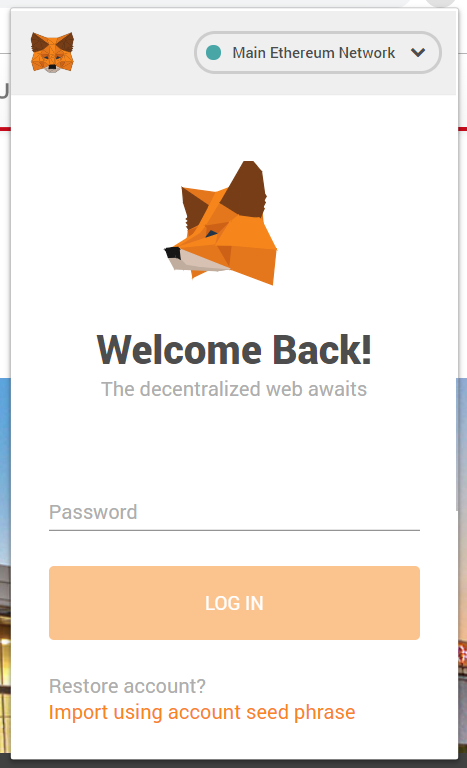
\includegraphics[scale=0.6]{images/metamasklogin.png}
\caption{Loging into the ethereum network}
\end{figure}

\subsubsection{Results}
\textbf{Viewing Results}\\~\\
This page can be accessed by a logged in student or an administrative assistant. The student can only view his/her results whereas the administrative assistant can view the results of various students.
\textbf{Manipulating results}\\~\\
In addtion to viewing results of various students, the adminsstrative assistant can also add/edit students’ results.

\section{Tests}
\subsection{Introduction}
The purpose of this section is to present the test cases used to test and validate the functionality of the Students' Results system's features.
\subsection{Scope}
To validate all the known functions of the Students' Results handler.
\subsection{Requirements}
The requirements for the tests are listed below, as they were derived and given in Chapter 4 of this report.\\\\
\textbf{User Requirements}
\begin{enumerate}
\item[U.1] Allow an administrative assistant enter students’ results.
\item[U.2] Allow students to access their results without being able to change them.
\item[U.3] Provide for students to easily share their results information with employers.
\item[U.4] Allow employers to easily verify students' results.
\end{enumerate}
\textbf{Functional Requirements}
\begin{enumerate}
\item[F.1] Ensure user authentication through login.
\item[F.2] Reject addition of inaccurate results.
\item[F.3] Ensure that the students’ results are not altered.
\item[F.4] Ensure students' transcript can be saved locally.
\item[F.5] Uploading transcript to IPFS.
\item[F.6] Saving IPFS hash to the blockchain.
\end{enumerate}
\textbf{Non-Functional Requirements}
\begin{enumerate}
\item[N.1] The system must verify any addition to the blockchain.
\item[N.2] The system must notify the system administrator incase of any unauthorized / failed transactions.
\end{enumerate}

\subsection{Test Cases}
% Please add the following required packages to your document preamble:
% \usepackage[table,xcdraw]{xcolor}
% If you use beamer only pass "xcolor=table" option, i.e. \documentclass[xcolor=table]{beamer}
% \usepackage[normalem]{ulem}
% \useunder{\uline}{\ul}{}
% \usepackage{longtable}
% Note: It may be necessary to compile the document several times to get a multi-page table to line up properly
\begin{longtable}{|p{0.5cm}|p{4cm}|p{2cm}|p{2cm}|p{3cm}|p{0.6cm}|}
\hline
\rowcolor[HTML]{010066} 
{\color[HTML]{FFFFFF} {\ul \textbf{Test ID}}} & {\color[HTML]{FFFFFF} {\ul \textbf{Test Case}}} & {\color[HTML]{FFFFFF} {\ul \textbf{Pre-conditions}}} & {\color[HTML]{FFFFFF} {\ul \textbf{Steps}}} & {\color[HTML]{FFFFFF} {\ul \textbf{Expected Output}}} & {\color[HTML]{FFFFFF} {\ul \textbf{Result}}} \\ \hline
\endfirsthead
%
\multicolumn{6}{c}%
{{\bfseries Table \thetable\ continued from previous page}} \\
\hline
\rowcolor[HTML]{010066} 
{\color[HTML]{FFFFFF} {\ul \textbf{Test ID}}} & {\color[HTML]{FFFFFF} {\ul \textbf{Test Case Description}}} & {\color[HTML]{FFFFFF} {\ul \textbf{Pre-conditions}}} & {\color[HTML]{FFFFFF} {\ul \textbf{Test Procedure}}} & {\color[HTML]{FFFFFF} {\ul \textbf{Expected Output}}} & {\color[HTML]{FFFFFF} {\ul \textbf{Result}}} \\ \hline
\endhead
%
\rowcolor[HTML]{9AFF99} 
\multicolumn{6}{|l|}{\cellcolor[HTML]{9AFF99}USER REQUIREMENTS} \\ \hline
U.1 & Allow Admininistrator assistant to enter student's results & Administrator must be logged in, Student Must be registered in system & Select Course, Select Year, Enter Student Name, Enter results & Results added to the databaseNotification for successfully entering results & Pass \\ \hline
U.2 & Allow students to access their results without being able to change them. & Student must be registered. Student must be logged in & Enters Student ID, View Results & Results displayed if student ID entered is valid,  Display an alert if Student ID is invalid & Pass \\ \hline
U.3 & Provide for students to easily share their transcripts with employers. & Student transcript is uploaded to IPFS & Create a URL for the transcript & Access the Transcript via Internet & Pass \\ \hline
\rowcolor[HTML]{9AFF99} 
\multicolumn{6}{|l|}{\cellcolor[HTML]{9AFF99}FUNCTIONAL REQUIREMENTS} \\ \hline
F.1 & Ensure user authentication through login, Case 1 - correct name and password, Case 2 - correct name and incorrect password, Case 3 - incorrect name and correct password, Case 4 - both name and password incorrect & User must be registered & Launch the app, Enter name, Enter password, Click Submit & Case 1 - User proceeds to dashboard, Cases 2, 3, 4 - Alert user and prevent log in & Pass \\ \hline
F.2 & Reject addition of inaccurate results, Case - Add mark \textgreater 100\% & User must be administrator & Log in, Select Student, Select Add Result & Alert user of incorrect mark entered & Pass \\ \hline
F.3 & Ensure that the students’ results are not altered, Case - Attempt to alter results & User must be Student & Log in, Try accessing database & Database should not be accessible to student & Pass \\ \hline
F.4 & Ensure students' transcript can be saved locally, Case - Downloading PDF format of transcript & User must  be logged in & Log In. Click Download button & Should download a PDF document & Pass \\ \hline
F.5 & Uploading transcript to IPFS. & User must be administrator, Transcript must be in PDF format & Save result as PDF, Ensure internet connection, Click Upload to IPFS & Create IPFS hash for the PDF and display transcript's URL & Pass \\ \hline
F.6 & Saving IPFS hash to the blockchain. & User must be administrator, User must be having an ethereum account and etherem wallet, Browser must be having MetaMask & Launch app, Accept MetaMask connection request, Click to Save hash to block chain, Accept MetaMask transaction request & Hash upload to Ethereum, Ethereum gas deduction - Wallet updated & Fail \\ \hline
\rowcolor[HTML]{9AFF99} 
\multicolumn{6}{|l|}{\cellcolor[HTML]{9AFF99}NON FUNCTIONAL REQUIREMENTS} \\ \hline
N.1 & The system must verify any addition to the blockchain. & User clicks upload to blockchain &  & Notify user using metamask transaction notification & Pass \\ \hline
N.2 & The system must notify the system administrator incase of any unauthorized / failed transactions. & Low Account Balance of ethereum wallet & User clicks upload to blockchain & Motify user through MetaMask notification & Pass \\ \hline
\caption{Table showing test cases for the system}
\label{Table 1}\\
\end{longtable}